\section{Projection Lab: seeing map distortion}\label{sec:p1}

\subsection{Purpose}

Most of us learned what the world looks like from Mercator maps, where Greenland appears about as large as Africa. Every flat map has to distort the round Earth somehow, but few people know how, or that other world maps make different trade-offs. Projection Lab is meant for everyday users rather than GIS experts: one world map with a slider that morphs smoothly from Mercator to Eckert IV, an equal-area projection (\cref{fig:p1-endpoints}). Watching Greenland, Canada and Russia shrink while Africa keeps its size makes the distortion visible without any formulas. Clicking a country shows how much Mercator exaggerates its area, and a short ``Method'' section explains the ideas in plain language.

\begin{figure}[htbp]
\centering
\begin{subfigure}{0.49\textwidth}
  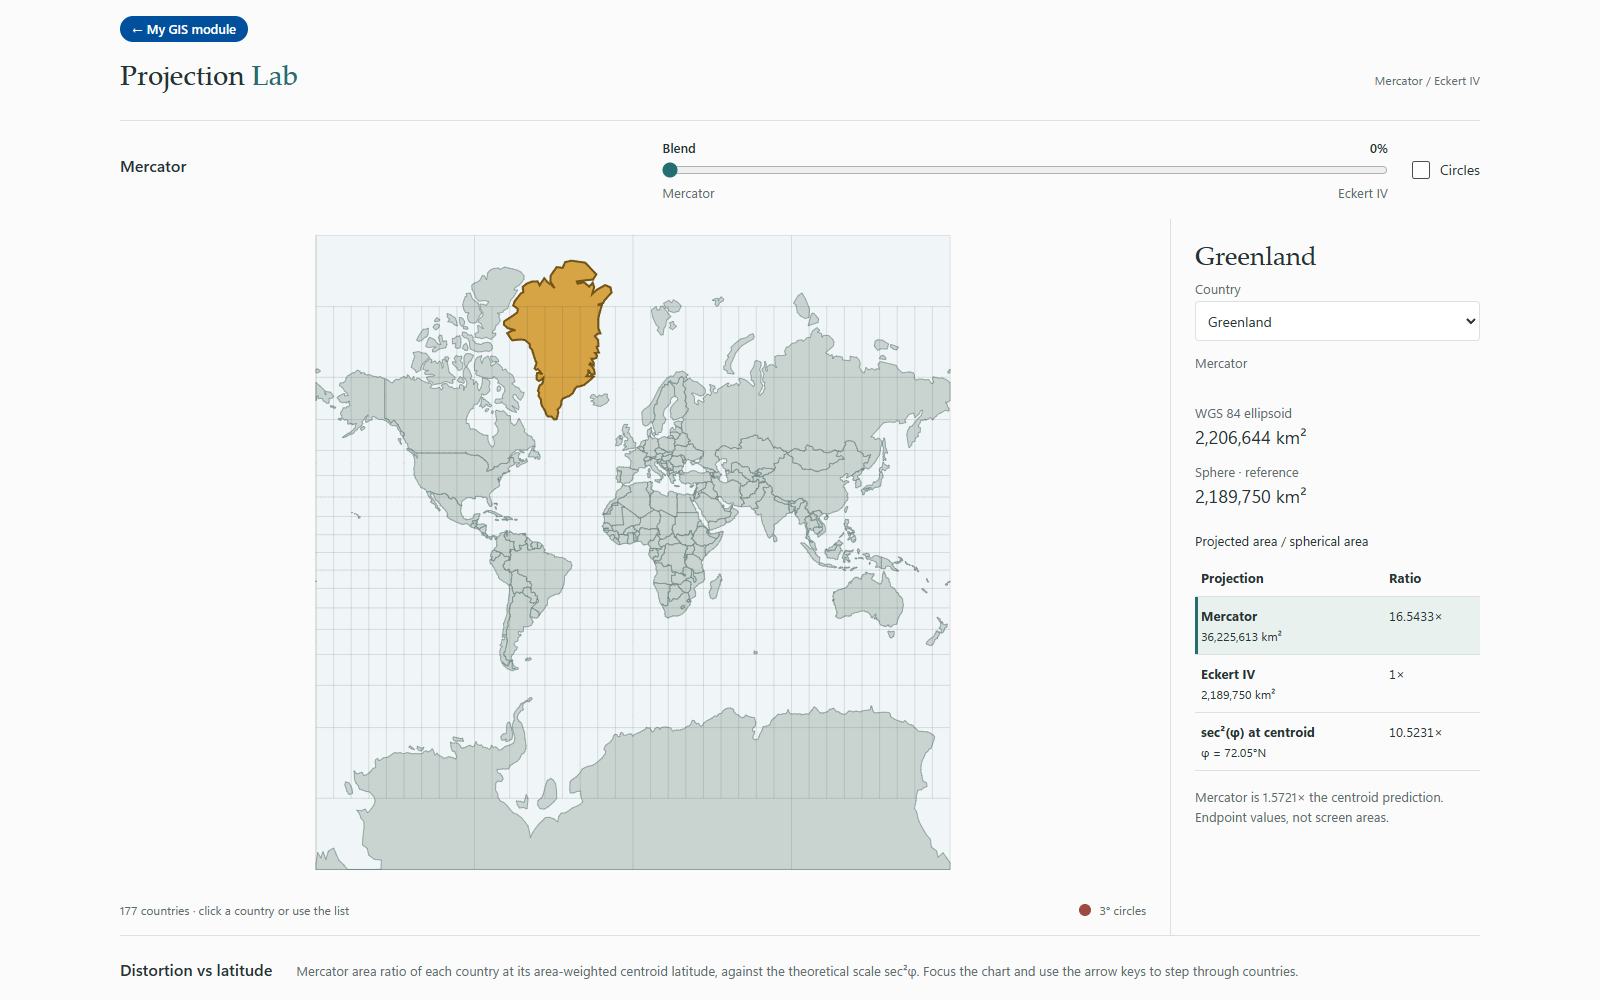
\includegraphics[width=\linewidth]{project-1-01-mercator.png}
  \caption{Mercator}
\end{subfigure}\hfill
\begin{subfigure}{0.49\textwidth}
  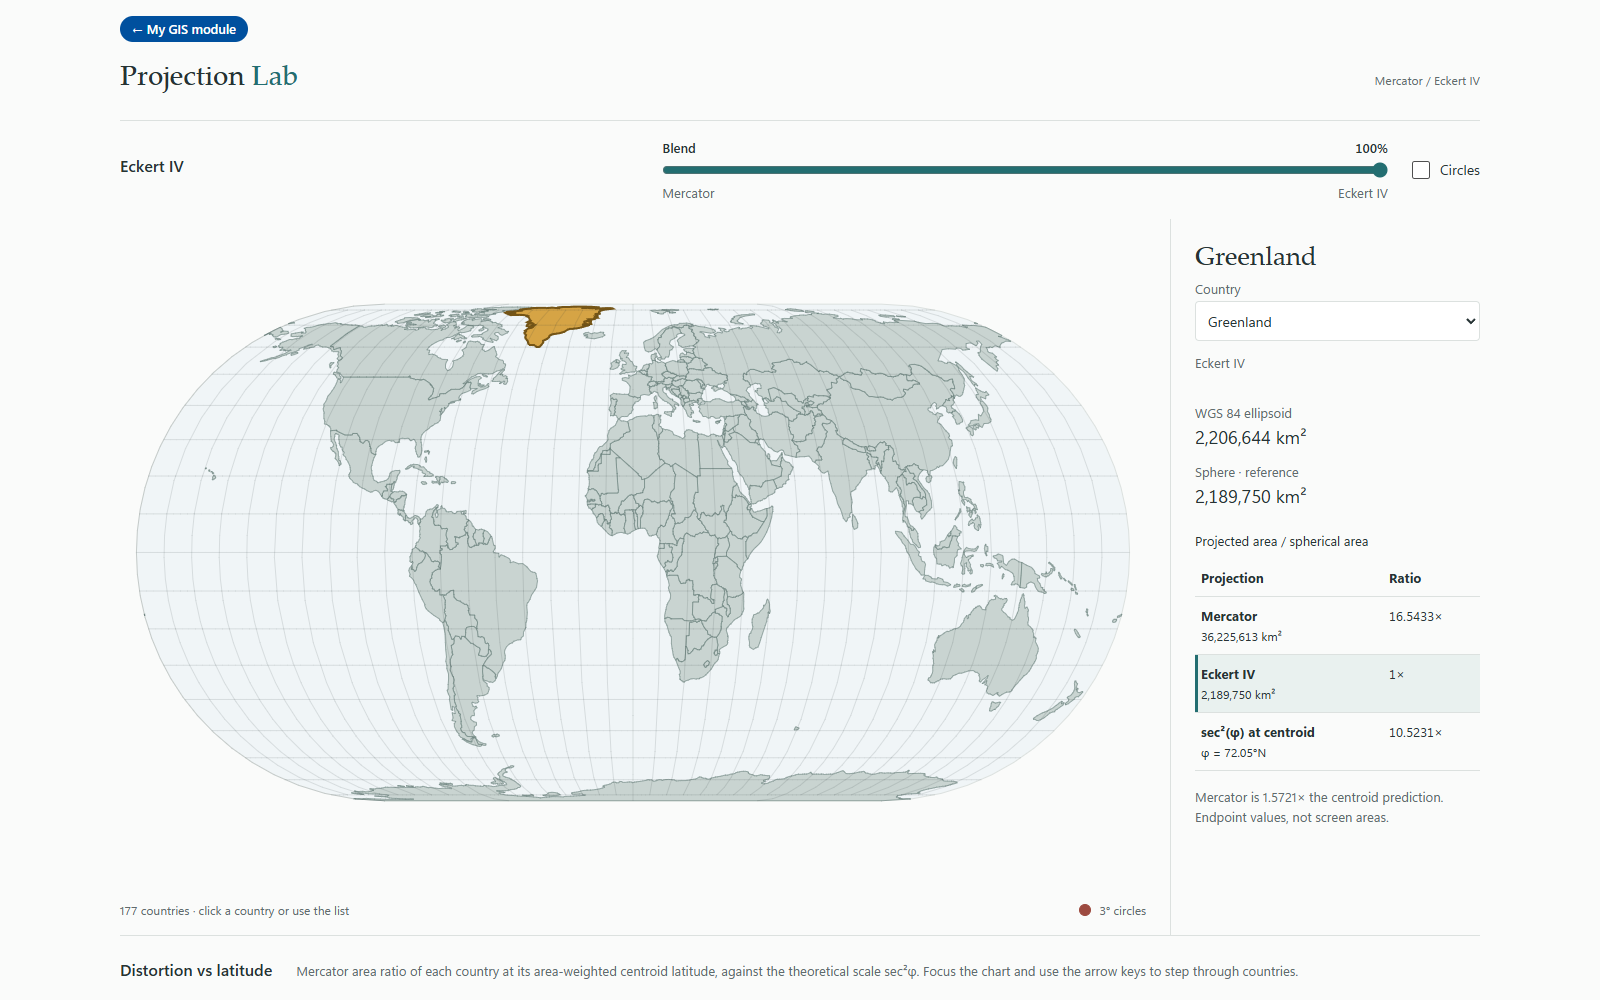
\includegraphics[width=\linewidth]{project-1-02-eckert-iv.png}
  \caption{Eckert IV (equal-area)}
\end{subfigure}
\caption{The two ends of the slider, with Greenland selected. In Mercator, Greenland is shown about 16.5 times too large; in Eckert IV it has its true relative size. Country boundaries: Natural Earth (public domain).}
\label{fig:p1-endpoints}
\end{figure}

\subsection{What I built}

\begin{itemize}
  \item A morphing world map with a blend slider, drawn in the browser with D3.
  \item Red ``distortion circles'': 30 circles of the same size on the globe, drawn through the current projection, as a simple version of Tissot's indicatrix (\cref{fig:p1-blend}). In Mercator they stay round but grow towards the poles; in Eckert IV they keep their area but get squashed.
  \item A panel for the selected country, comparing its true area with its Mercator and Eckert IV areas.
  \item A chart of distortion against latitude for all 177 countries, which shows the pattern at a glance: the farther from the equator, the larger the exaggeration.
\end{itemize}

\begin{figure}[htbp]
\centering
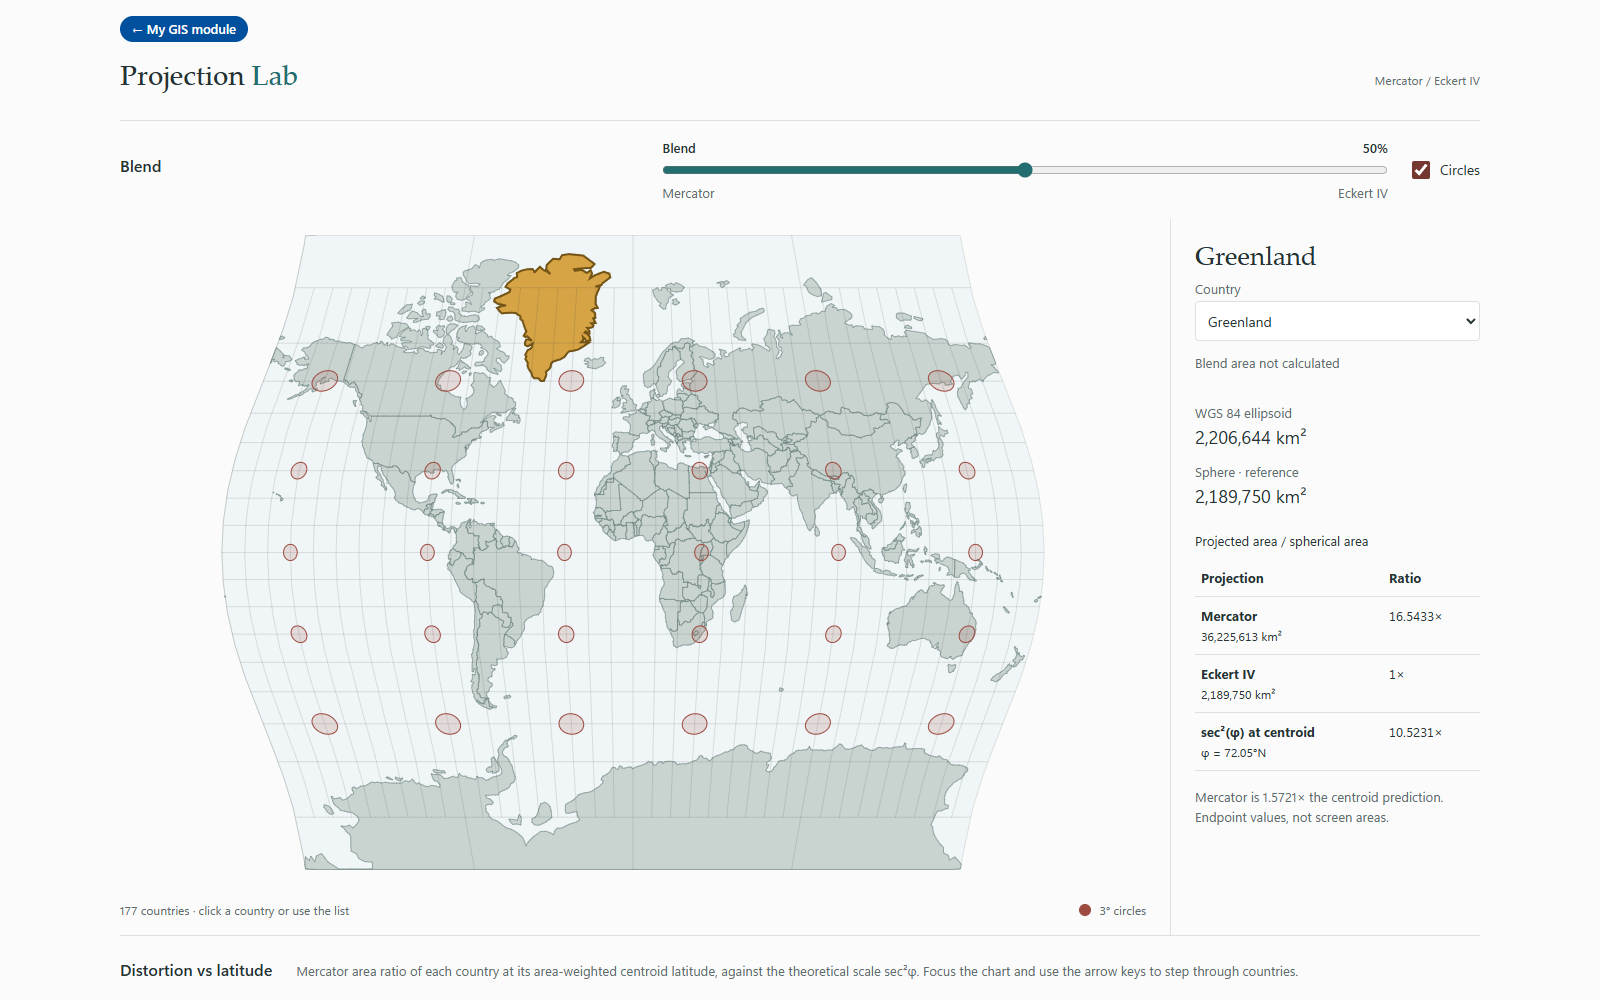
\includegraphics[width=0.8\textwidth]{project-1-03-blend-50-circles.png}
\caption{Halfway between the projections, with the distortion circles. All circles are the same size on the globe; how they are drawn shows where the map stretches. Data: Natural Earth.}
\label{fig:p1-blend}
\end{figure}

\subsection{Technologies and what I learned}

\paragraph{D3 and map projections.} The frontend uses React and d3-geo \citep{d3}. I learned that a projection in D3 is just a function from longitude and latitude to screen coordinates, so two projections can be blended by interpolating their outputs. The blend itself is neither conformal nor equal-area, which is why the app only reports areas at the two ends of the slider.

\paragraph{The idea behind the distortion.} Building the area calculation made the theory concrete. Mercator preserves angles and local shapes, but stretches the map by the same factor in both directions, and that factor grows with latitude ($\sec\varphi$). Area is therefore stretched by $\sec^2\varphi$: not at all at the equator, four times at 60\dg{}, and without limit at the poles, which is why Mercator maps are cut off around 85\dg{}. An equal-area projection like Eckert IV keeps every area correct but has to bend shapes instead. No flat map can do both, and seeing this happen on the slider is the main message of the app.

\paragraph{PostGIS, pyproj and Shapely.} The country data (Natural Earth, 1:110m \citep{naturalearth}) is stored in PostgreSQL with PostGIS. Here I learned the difference between PostGIS \code{geometry} and \code{geography}: the same area query returns square degrees on one and square metres on the other. I also met real data problems: two countries (the USA and Sudan) had invalid geometries that had to be repaired, Antarctica reaches the pole where Mercator is undefined, and some countries cross the 180\dg{} meridian. The areas themselves are computed once in Python with pyproj \citep{pyproj} and Shapely \citep{shapely} and stored in the database.

\paragraph{FastAPI, Docker and a static version.} A small FastAPI service \citep{fastapi} serves the data to the frontend, and Docker Compose runs the database, the API and the web server together, so the whole stack can be rebuilt from scratch with a few commands. GitHub Pages cannot run a backend, so I also added a static mode in which the frontend reads exported JSON files instead of the API. This taught me to think about where an app will run before deciding how it gets its data.

\paragraph{Working as a learner.} The first phases (September) were done in tutoring mode: I wrote the code myself with the assistant explaining and reviewing. The goals were to rebuild my coding fluency, practise debugging and get into the habit of reading official documentation (D3, PostGIS, PROJ, FastAPI). Extending the project from Greenland to every country was done later, in the sprint, with the assistant writing the code.

\subsection{Result}

The finished app makes the distortion easy to see: Greenland is shown about 16.5 times too large in Mercator, while countries near the equator are barely affected. A main limitation is that the areas describe simplified 1:110m boundaries, not official national areas. The map itself is also not fully usable with a keyboard or screen reader.
